% ICASSP 2027 submission draft.
% REQUIRED BEFORE SUBMISSION: replace the author block below with the legal
% author name(s), affiliation(s), and email address(es). ICASSP is not blind.
\documentclass{article}
\makeatletter
\def\input@path{{../../.submission_reqiurement/}}
\makeatother
\usepackage{spconf,amsmath,graphicx,booktabs,url}
\usepackage{newtxtext,newtxmath}
\usepackage[hidelinks]{hyperref}
\usepackage{balance}
\urlstyle{same}
\let\standardthebibliography\thebibliography
\renewcommand{\thebibliography}[1]{%
  \standardthebibliography{#1}\setlength{\itemsep}{-0.2pt}}

\title{GGUF-METADATA PREDICTION OF SINGLE-SEQUENCE LLAMA.CPP THROUGHPUT ACROSS THREE SYSTEMS}
\name{Author Name}
\address{Affiliation\\author@example.com}

\begin{document}
\ninept
\setlength{\emergencystretch}{1em}
\maketitle

\begin{abstract}
We predict single-sequence model throughput from GGUF metadata using
roofline-shaped predictors with quantization-specific scale factors fitted on
reference models.  The scored cohort comprises 318 phase--depth measurements
from 53 host--file configurations on two Apple M4 Max systems and an NVIDIA RTX
5080.  On host-specific held-out sets of four, five, and two configurations, an
active-parameter decode model obtains 13.1\%, 14.4\%, and 36.1\% mean absolute
percentage error (MAPE), versus 49.4\%, 55.3\%, and 51.9\% when charging total
parameters.  Leave-one-host-out coefficients fitted on the other two systems
yield 11.6\%, 16.8\%, and 36.0\% test MAPE.  A low-bit model ladder changes
ordering across runtime stacks.  The P2 prefill baseline gives 18.7\%, 22.2\%,
and 108.2\% test MAPE.  GGUF structure helps on all three systems, but fitted
efficiencies are not universal.
\end{abstract}

\begin{keywords}
large language models, performance prediction, llama.cpp, GGUF,
mixture of experts
\end{keywords}

\section{Introduction}
\label{sec:intro}

Choosing a local language model often requires benchmarking several
multi-gigabyte GGUFs.  A predictor based on stored metadata would reduce
candidate executions relative to a lookup table; remote header-only acquisition
is outside our scope.  Three effects complicate a raw memory roofline
\cite{williams2009roofline}: quantized kernels attain different fractions
of peak bandwidth, mixture-of-experts (MoE) models store many more weights than
they activate per token, and hybrid architectures allocate key--value (KV) state differently
in global, sliding-window, and recurrent layers.

We ask which parts of such a predictor transfer across model families and
hardware.  Our first contribution is a host-adapted decode model whose target
features---file size, tensor shapes, expert routing, and per-layer attention
metadata---are available before inference.  We evaluate a frozen family split
on two unified-memory Apple systems and a discrete NVIDIA GPU.  Second, we
isolate the benefit of activated-parameter and per-layer KV accounting.  Third,
we report transfer limits rather than hiding them in a pooled score: one-term
coefficients only partly transfer, low-bit behavior varies by system, and
the tested prefill model does not replicate on RTX.

LLMCompass explores accelerator design \cite{zhang2024llmcompass}.  Vidur
combines profiling with serving simulation \cite{agrawal2024vidur}.
RooflineBench and LIMINAL apply hardware-aware analysis to LLM inference
\cite{bi2026rooflinebench,davies2025liminal}.
MoE-CAP argues that sparse utilization should be measured over activated rather
than stored parameters \cite{jiang2025moecap}; we test the predictive effect of
that accounting.  Benazir and Lin characterize quantization and memory behavior
on Apple Silicon \cite{benazir2025apple}.  Our narrower estimator targets
unmeasured single-sequence GGUF families from metadata plus a small reference
set, followed by an explicit cross-system falsification test.  Measurements use \texttt{llama-bench} from
\texttt{llama.cpp} \cite{gerganov2023llamacpp}; GGUF parsing follows its format
specification \cite{ggufspec}.

\begin{figure*}[!t]
  \centering
  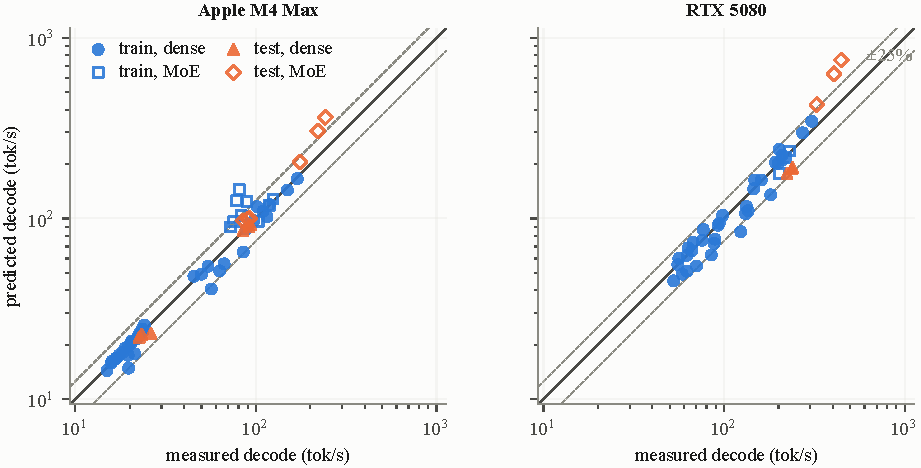
\includegraphics[width=\textwidth]{../../figures/paper/fig1_accuracy.pdf}
  \caption{B2 decode predictions, separated by host.  The 159 points comprise
  57 MacBook, 60 Studio, and 42 RTX observations, with 126 training and 33 held-out; dashed
  lines mark $\pm25\%$.  Open markers are MoE and orange markers are held-out.}
  \label{fig:accuracy}
\end{figure*}

\section{Predictor}
\label{sec:model}

Let measured $T_d(c)$ and $T_p(c)$ denote decode and prefill throughput.  Let
$S$ be GGUF file size, $P$ and $P_a$ total and activated parameter counts,
$B_h$ measured bandwidth on host $h$, and $c$ existing-prefix depth.  We model
bytes per generated token and decode tokens per second as
\begin{align}
 D(c)&=S\frac{P_a}{P}+K(c), &
 \widehat T_d(c)&=\eta_{h,q}\frac{B_h}{D(c)}, \label{eq:decode}\\[-2mm]
 K(c)&=\sum_i2h_i d_i\min(c,w_i)b_{\rm KV}+S_{\rm state}. \label{eq:kv}
\end{align}
Here $q$ is quantization format, $h_i$ and $d_i$ are a layer's KV-head count
and head dimension, $w_i$ is its window ($\infty$ for global attention), and
$b_{\rm KV}=2$ bytes per cached scalar for the fixed F16 cache, and
$S_{\rm state}$ is fixed recurrent-state traffic.  Recurrent layers set $h_i=0$.
Tensor dimensions and expert-routing fields
estimate $P_a$; if an expert bank has $P_e$ weights, $E$
experts, and $k$ selected experts, then
$P_a=P-P_e+(k/E)P_e$.  Dense models have $P_a=P$.

For each $(h,q)$, $\eta_{h,q}$ is the median of
$T_dD/B_h$ over training rows; an unseen format uses the host-wide median.
This ratio-space fit prevents the fastest small
models from dominating least squares.  It is an empirical scale factor, not
literal utilization: $S P_a/P$ assumes file-wide average bytes per parameter,
and both file bytes and the copy benchmark are traffic proxies, so
$\eta$ may exceed one.  B0 is the unfitted total-size roofline
$B_h/(S+K)$; B1 fits $\eta_{h,q}$ but still charges total weights; B2 uses
Eqs.~\eqref{eq:decode}--\eqref{eq:kv}.  Comparing B1 with B2 isolates
active-weight accounting while holding the fitting rule fixed.  Because $B_h$
cancels after same-host fitting, it affects B0 and cross-host substitution, not
target-fitted B1/B2 accuracy; $F_h$ analogously cancels for P1/P2.

We also test the deliberately simple zero-prefix prefill model
\begin{equation}
 \widehat T_p=\phi_{h,q}\frac{F_h}{2P_a}, \label{eq:prefill}
\end{equation}
where $F_h$ is calibrated matrix throughput.  For each depth-zero training row,
we back-solve $r=T_p(2P_a)/F_h$.  P1 sets $\phi_h$ to the median $r$ for host
$h$; P2 uses the median within each host--quantization group.  An unseen
quantization falls back to the median of that host's fitted group coefficients.
Neither model contains an existing-prefix term, so greater depths are scope
tests, not part of the fit.

\begin{figure*}[!t]
  \centering
  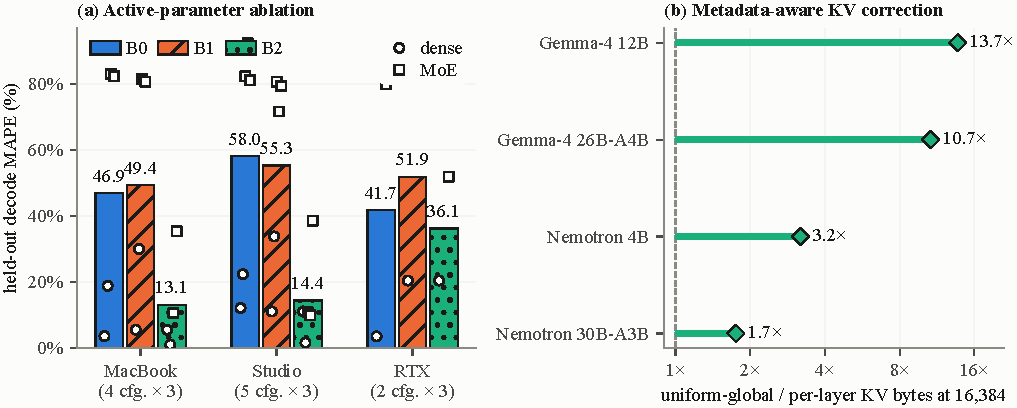
\includegraphics[width=\textwidth]{../../figures/paper/fig2_mechanisms.pdf}
  \caption{Structural corrections.  (a) Bars are host-specific held-out MAPE;
  overlaid points are per-configuration means across three depths and expose
  the four-, five-, and two-configuration test sizes.  (b) From GGUF metadata, treating every layer
  as global overstates 16K KV bytes by as much as $13.7\times$.}
  \label{fig:mechanisms}
\end{figure*}

\begin{figure*}[!t]
  \centering
  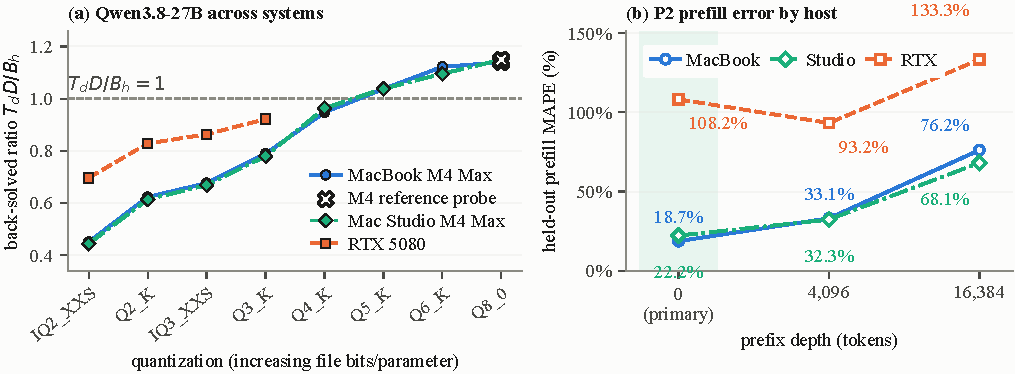
\includegraphics[width=\textwidth]{../../figures/paper/fig3_scope.pdf}
  \caption{Transfer diagnostics.  (a) The back-solved depth-zero ratio
  $T_dD/B_h$ for one Qwen family varies across systems; RTX covers the first
  four formats.  The crossed Apple Q8 points are historical reference probes,
  shown for ladder context but excluded from fitting and scoring.  (b) P2
  prefill error is host-specific, remains poor on RTX, and rises by 16K.}
  \label{fig:scope}
\end{figure*}

\section{Experimental method}
\label{sec:method}

The hosts are a 64-GB MacBook Pro M4 Max and a 128-GB Mac Studio M4 Max, each
using 12 performance-core threads, plus an RTX 5080 with 16,302~MiB reported
VRAM, CUDA, and 16 threads.  Their device-copy/FP16 matrix calibrations are
380.1~GB/s and 13.95~TFLOP/s, 396.7~GB/s and 15.00~TFLOP/s, and 801.1~GB/s and
118.83~TFLOP/s, respectively.  The Studio binary is from the hash-recorded
official b10794 archive.  The managed RTX directory is labeled b10794, but its
version query returned usage text; the legacy MacBook revision was not recovered.

The shared manifest has 23 GGUF files.  The MacBook produced 22 successful
grids; after three pre-specified reference-probe exclusions, it contributes 15
training and four held-out configurations.  Studio completed all 23 grids and
contributes 15 and five after the same exclusions.  RTX covers 14 matching files,
split 12 and two.  The 53 scored configurations span 22 files; each held-out set
contains dense and MoE families absent from training, though RTX remains a small
replication.  Results are therefore host-separated.  Splits are fixed by base
family before fitting.  The 63.39-GB gpt-oss-120B file produced two prompt-batch
failures on MacBook, not a demonstrated out-of-memory failure, and a complete
grid on Studio.  The supplement lists every file, source URL, revision, and byte
size; source organizations are cited here \cite{unsloth_models,lmstudio_models,
ggmlorg_models,google_models,bartowski_models}.

All reported throughput is single-sequence.  Each configuration runs in a
fresh process.  At prefix depths 0, 4096, and 16384, \texttt{llama-bench}
reports separate 512-token prompt-processing and 128-token generation
microbenchmarks, not one end-to-end request.  Runs use flash attention, F16 K/V,
five repetitions, and 45~s settling.  The requested GPU-layer count is 99.  Physical
RTX residency was not instrumented; Windows shared-memory spill therefore
cannot be excluded for the largest files.  The append-only data are reduced by
an atomic selector that prefers complete protocol rows and then lower decode
coefficient of variation (CV)
and pre-run load, without inspecting prediction residuals.

The stability gate applies to decode.  Across all selected rows, median decode
CV is 0.83\%, 0.42\%, and 0.43\% on MacBook, Studio, and RTX; maxima are 3.04\%,
2.30\%, and 1.65\%.  Prefill was not gated: 8/66, 0/69, and 29/42 rows exceed 3\%,
with maxima 4.84\%, 0.96\%, and 39.2\%.  We retain them and give a median-sample
sensitivity below.  Each decode configuration contributes its three depths.

\section{Results}
\label{sec:results}

\begin{table}[t]
\centering
\caption{Host-separated MAPE (\%).  ``Cfg.'' is the number of model--format
configurations; decode includes three depths per configuration, while P1/P2
are scored at depth zero.}
\label{tab:error}
\setlength{\tabcolsep}{3.0pt}
\begin{tabular}{@{}llrrrrr@{}}
\toprule
Host & Split (cfg.) & B0 & B1 & B2 & P1 & P2\\
\midrule
MacBook & train (15) & 33.6 & 15.8 & \textbf{10.4} & 6.8 & \textbf{4.1}\\
        & test (4)   & 46.9 & 49.4 & \textbf{13.1} & 22.7 & \textbf{18.7}\\
Studio & train (15) & 33.0 & 17.8 & \textbf{12.4} & 7.0 & \textbf{4.3}\\
       & test (5)   & 58.0 & 55.3 & \textbf{14.4} & 28.0 & \textbf{22.2}\\
RTX 5080 & train (12) & 20.3 & \textbf{9.8} & 10.1 & 14.5 & \textbf{5.9}\\
         & test (2)   & 41.7 & 51.9 & \textbf{36.1} & 124.5 & 108.2\\
\bottomrule
\end{tabular}
\end{table}

\subsection{Host-adapted decode}

Figure~\ref{fig:accuracy} and Table~\ref{tab:error} show the primary result.
B2 train/test MAPE is 10.4/13.1\% on MacBook, 12.4/14.4\% on Studio, and
10.1/36.1\% on RTX.  RTX test median/maximum error is 25.8/69.0\%.  On the exact
two-file intersection shared by all hosts, MAPE is 18.2\%, 20.1\%, and 36.1\%,
respectively.  RTX remains the smallest replication, but B2 improves on B1 for
every held-out host.

Active-weight accounting substantially improves the held-out aggregate
(Fig.~\ref{fig:mechanisms}a): B1 errors of 49.4\%, 55.3\%, and 51.9\% fall to
13.1\%, 14.4\%, and 36.1\%.  Capacity is controlled by stored parameters,
whereas per-token weight traffic is closer to activated parameters.  Separately,
Eq.~\eqref{eq:kv} avoids the
$10.7$--$13.7\times$ cache overestimates produced by a uniform-global formula
for the two Gemma-4 examples (Fig.~\ref{fig:mechanisms}b).  After refitting each
variant, per-layer rather than uniform-global KV lowers held-out MAPE from
21.2\% to 13.1\% on MacBook, 21.0\% to 14.4\% on Studio, and 37.9\% to 36.1\% on RTX.

\begin{figure*}[!t]
  \centering
  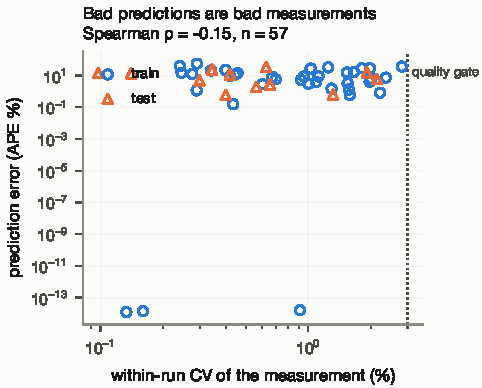
\includegraphics[width=\textwidth]{../../figures/paper/fig8_quality_vs_error.pdf}
  \caption{Measurement diagnostics.  (a) Host-separated decode CV shows no obvious descriptive association
  with B2 error across 159 scored rows; the dotted line is the 3\% target.
  (b) Row-level CV distributions use all 354 selected rows, including 36 Apple
  reference-probe rows; labels count rows above the target.  The gate covered
  decode (D), not prefill (P).}
  \label{fig:quality}
\end{figure*}

\subsection{Cross-host transfer is incomplete}

Separate fitting should not be confused with hardware generalization.  In a
leave-one-host-out diagnostic, B2 coefficients are fitted independently on the
other two machines, given equal source-host weight, and paired with the target's
calibrated bandwidth.  All-target MAPE is 14.5\%, 15.4\%, and 20.8\% for 57
MacBook, 60 Studio, and 42 RTX rows; target-fitted B2 gives 11.0\%, 12.9\%, and
13.8\%.  Restricted to target test families, transfer gives 11.6\%, 16.8\%, and
36.0\%, close to target-fitted 13.1\%, 14.4\%, and 36.1\%.  This test is easier
than simultaneous model-and-host holdout because most target files occur on a
source host.

The 14 three-way matched configurations span eight base families and weight each
format equally.  Across 22 MacBook--Studio matches, Studio/MacBook geometric-mean
zero-prefix throughput is $1.02\times$ for both decode and prefill.  RTX/MacBook
is $2.15\times$ for decode, near the $2.11\times$ copy-bandwidth ratio, and
$7.21\times$ for prefill versus an $8.52\times$ compute ratio.  Configuration-level
decode ratios span $1.76$--$3.26\times$, ruling out one universal multiplier.

The near-family Qwen3.8-27B ladder varies across the three host/runtime stacks
(Fig.~\ref{fig:scope}a).  IQ2 has 1.55\% fewer parameters and one fewer layer.
On both Apple hosts, Q2 is only 2.2\% faster than IQ2 at depth zero, whereas on
RTX, IQ2 is 13.7\% faster.  Across the three conventional Q4/Q8 pairs, Q4 is
$1.32$--$1.43\times$ faster on MacBook, $1.29$--$1.41\times$ on Studio, and
$1.37$--$1.49\times$ on RTX, while its
prefill rate is usually slightly lower.  File compression alone therefore does
not specify kernel efficiency.

\subsection{Prefill is a negative result}

P1/P2 held-out zero-prefix MAPE is 22.7/18.7\% on MacBook, 28.0/22.2\% on
Studio, and 124.5/108.2\% on RTX (Fig.~\ref{fig:scope}b).
The RTX result is not solely the 39.2\%-CV Ling cell:
replacing every cell mean by its five-sample median and refitting still gives
85.5\%.  At 16K, where Eq.~\eqref{eq:prefill} omits prefix-dependent work, test
error rises to 76.2\% on MacBook, 68.1\% on Studio, and 133.3\% on RTX.  Most
host--quantization groups contain only one training configuration, so the
per-format coefficients are weakly identified and P2's low 4.1--5.9\% training
errors are partly resubstitution.  We consequently treat prefill as
unsupported under this protocol, not as a successful second regime.

\subsection{Protocol and robustness checks}

Decode behaves more consistently than its largest residuals.  Every scored
configuration slows monotonically with context.  B2 held-out MAPE falls from
17.9\% to 8.6\% between depth zero and 16K on MacBook, 18.1\% to 9.7\% on Studio,
and 44.5\% to 25.6\% on RTX.  Across all 159 scored decode rows, within-run CV
shows no obvious descriptive association with residual error (pooled Spearman
$\rho=-0.05$; host values are $-0.14$, $0.01$, and $0.16$;
Fig.~\ref{fig:quality}), and within-run scatter is much smaller than the largest
residuals.

Correlated depth rows and absent Studio/RTX between-run studies limit noise
attribution.  The supplement reports a rejected output-projection extension.

\section{Limitations and conclusion}
\label{sec:conclusion}

The RTX held-out set has only two Q4\_K\_M files and no independent between-run
repeatability campaign; acquisition spans two sessions.  Quantization formats
often have one training family, IQ2's Qwen file has 1.55\% fewer parameters
than the rest of that ladder, and execution order was not randomized.  The
largest RTX analytical working set exceeds reported VRAM before graph buffers,
so requested full layer offload is not proof of physical residency.  No GPU
clock, power, or spill telemetry was recorded.  Studio files were SHA-verified
against repository LFS identifiers; equivalent immutable captures are
unavailable for the legacy hosts.  These limitations preclude a universal runtime
accuracy claim.  All error summaries are descriptive, not population confidence
estimates.  The $SP_a/P$ proxy also scales shared tensors with expert tensors
and assumes balanced $k/E$ routing; tensor-level active-byte validation was
unavailable.  No learning curve establishes how many reference configurations
are sufficient.

Within that boundary, active-weight and metadata-aware KV corrections reduce
held-out decode error in all three cohorts; source-host-balanced coefficients
remain close after target bandwidth calibration.  Host/runtime-stack differences
in low-bit behavior argue against a universal coefficient; differing runtime
versions and IQ2's slightly different architecture remain confounds.  Next work
should record residency and broaden the cohort.

\clearpage
\setlength{\emergencystretch}{1.5em}
\Urlmuskip=0mu plus 1mu
\balance
\bibliographystyle{../../.submission_reqiurement/IEEEbib}
\bibliography{references}

\end{document}
